
% Formatka dla raportów projektowych dla Koła Naukowego KoNaR 
% Autor: Bartosz Kolasa
% Edycja: Michał Swoboda
% Edycja2: Bartłomiej Kurosz
% Treść: Bartłomiej Kurosz

%-------------------------------------
% Definicja klasy dokumentu
\documentclass[12pt,a4paper]{article}

%------------------------------------
% 			Pakiety
\usepackage[utf8x]{inputenc}
\usepackage{ucs}
\usepackage[MeX]{polski}
\usepackage{fancyhdr}
\usepackage{amsmath}
\usepackage{amsfonts}
\usepackage{amssymb}
\usepackage[hidelinks]{hyperref}
\usepackage{graphicx}
\usepackage{amssymb}
\usepackage{subfig}
\usepackage{supertabular}
\usepackage{array}
\usepackage{tabularx}
\usepackage{hhline}
\usepackage{tabulary}
\usepackage{float}
\pagestyle{fancy}

%---------------------------------------
% 		Dodanie strony tytulowej do dokumentu

\renewcommand{\maketitle}{\begin{titlepage}

\begin{center}

\includegraphics[scale=1]{logo.png}
\vspace*{1cm}
\noindent \rule{\linewidth}{0.4mm}
\LARGE \textsc{Raport z Budowy Robota: \\ BD2} % Tutaj należy umieścić tytuł projektu 
\vspace*{0.5cm}
\rule{\linewidth}{0.4mm}
\vspace*{1cm}
\LARGE
\textsc{Wykonał: Szymon Czaja}  \\% W tym miejscu należy zamieścić 
\textsc{} \\
\large
\textsc{Na bazie projektu Biała Dama stworzonego przez Szymona Czaje i Marka Żyśko } \\ % W tym miejscu należy zamieścić 


\vspace*{2cm}
\textsc{Koło Naukowe Robotyków KoNaR }\\
\textsc{\url{www.konar.pwr.edu.pl}}\\
\textsc{\today}\\
\end{center}
\end{titlepage}
\newpage
} % W tym pliku należy w odpowiednim miejscu wpisać członków zespołu

%-----------------------------------------
% 		Poczatek dokumentu
\begin{document}
\maketitle % Komenda maktitle dodaje stronę tytułową do dokumentu głównego
\tableofcontents % Komenda tableofcontents dodaje spis treści do dokumentu głównego
\newpage % Komenda newpage przechodzi do nowej strony w dokumencie.

%------------------------------------------
%				Dokument wlasciwy
\section{Wstęp}
Na wstępie chciałem zaznaczyć że robot BD2 jest to odnowiona wersja Robota Biała-Dama którego robiłem na warsztatach robotycznych 2016. Ów robota robiłem we współpracy z Markiem Żyśko który był odpowiedzialny za wykonanie obudowy oraz koncept tego jak nasz robot pod względem mechanicznym ma wyglądać. Te właśnie rzeczy nie zostały wcale zmienione w mojej wersji robota na ten rok. BD2 jest moją osobistą wersją wspólnego projektu sprzed roku. Podstawowym celem projektu było zapoznanie się z podstawowymi zasadami konstrukcji
robota typu minisumo, poznanie najczęściej wykorzystywanych podzespołów,
programów typu CAD oraz środowisk programistycznych. W celu
obycia się z narzędziami wykorzystywanymi w praktyce ograniczono wykorzystywanie
gotowych części do niezbędnego minimum i większość konstrukcji
wykonano samodzielnie. Dodatkową motywacją była możliwość wstąpienia
do Koła naukowego KoNaR.


\section{Szczegóły konstrukcyjne}

Robot Biała Dama w pierwotnej wersji był inspirowany robotem 2week4u.
Jednak podczas prac wykorzystywaliśmy własne rozwiązania. Niektóre z nich
były dobrym pomysłem inne wręcz przeciwnie. BD2 natomiast Naprawiał niektóre błędy poprzednika oraz dodał takie możliwości jak sterowanie przez aplikacje bluetooth oraz czujniki białej linii.

\subsection{Mechanika}
Do zaprojektowania mechaniki robota wykorzystany został program Autodesk
Inventor Professional 2017. Z racji wykonywania większości części ręcznie
projekt został ograniczony do niezbędnego minimum czyli obudowy wykonanej
z czterech płaskich płyt stalowych zespawanych razem. Zostały również wycięte otwory na czujniki.

\begin{figure}[!]
\centering
\includegraphics[width=0.8\textwidth]{figures/obudowa}
\caption{obudowa  \label{fig:STM}}
\end{figure}

\subsubsection{Zawieszenie}
Zawieszenie wykonane zostało ze stalowej blachy o grubości 4 mm w celu
obniżenia środka ciężkości. Osadzenie silnikow na zawieszeniu pozwoliło
uniknąć dużych naprężeń na łączeniach płytki PCB z obudową o znacznie
większej masie.


\subsubsection{Pług}
Ze względu na niewłaściwy dobór materiału w zakupionym przez podwykonawcę
pługu zrezygnowano z wykorzystania popularnego noża do strugarek. Zamiast tego naostrzona została przednia blacha. Rozwiązanie to spełniało soja role raz lepiej raz gorzej jednak nigdy robot nie został całkowicie podbity co sugeruje że rozwiązanie to nie jest najgorszym pomysłem.

\subsubsection{Silniki}
Zastosowano dwa silniki firmy pololu z karbonowymi szczotkami oraz przekładnią
50:1. Silniki te są idealnym kompromisem miedzy mocą, a wymiarami
które w robotach klasy minisumo są bardzo ograniczone. Silniki Te jednak szybko się palą. Podczas testów zostały lekko nadpalone, co odbijało się negatywnie na mocy robota na zawodach.

\begin{figure}[!]
\centering
\includegraphics[width=0.8\textwidth]{figures/silniki}
\caption{silniki  \label{fig:STM}}
\end{figure}

\subsubsection{Koła}
Koła wykorzystane w robocie to hybryda drukowanych przestrzennie koła których autorem
jest Michał Burdka oraz kół z Botlandu. Po zawodach w 2016 wykonane przez Michała ogumienie się bardzo zniszczyło. Nie można jednak było wymienić całych kół ponieważ koła zamówione z Botlandu mają trochę inne wymiary i nie mieściły się w obudowie. W wyniku czego wykorzystałem felgi z starych kół i nowe ogumienie co bardzo pozytywnie wpłynęło na przyczepność robota.

\subsubsection{Podsumowanie Mechaniki}
Głównym błędem mechanicznym projektu było przeniesienie środka ciężkości robota bardzo blisko osi kół. Było to celowym zabiegiem w celu zminimalizowania strat energii podczas tarcia pługiem o podłoże. Poskutkowało to jednak małą przyległością pługa do ziemi w porównaniu z innymi konstrukcjami. W efekcie stosunkowo łatwo podbić naszego robota przez co często traci on szanse na wygraną.

\subsection{Elektronika}
Schemat Elektroniczny oraz Projekt płytki pcb wykonane zostały w darmowym programie KiCad. Wybór ów był podyktowany: prostotą programu, dostępnością oraz Tym że właśnie ten program był omawiany na warsztatach Robotycznych KoNaRu 2016.

\subsubsection{Zasilanie}
Robot zasilany jest baterią lipolu 7.4 V, bateria ta jest stosunkowo tania oraz ma bardzo dobrą wydajność prądową. Napięcie zostało podzielone na 5V i 3.3V dzięki dwóm dzielnikom napięć LM1117 który jest popularny w robotach tego typu i łatwo dostępny. Główny switch włącza zasilanie w całym obwodzie. Dioda Led informuje o obecności napięcia. 

\begin{figure}[!]
\centering
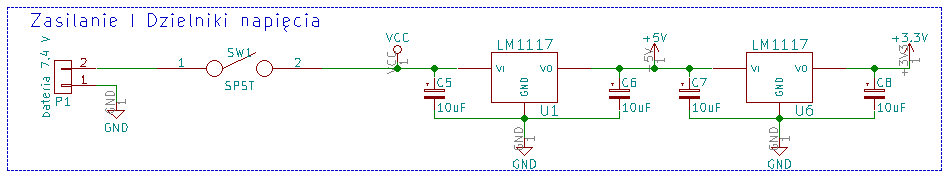
\includegraphics[width=0.8\textwidth]{figures/zasilanie}
\caption{schemat stabilizatorów napięcia  \label{fig:zasilanie}}
\end{figure}

\subsubsection{Mikrokontroler}
Mikrokontroler użyty w robocie jest to STM32F051C8T6 z maksymalnym taktowaniem 48 MHz. Wybrany został ten właśnie model przez wygodne i darmowe oprogramowanie do niego oraz niską cenę. Program STM32CubeMX pozwala bardzo szybko i łatwo skonfigurować odpowiednie piny, zegary i przerwania. System Workbench for STM32 jako środowisko programistyczne wraz z STMStudio jest wyśmienitym narzędziem które znacząco skraca czas szukania błędów i pozwala na lepsze zrozumienie kodu. 


\begin{figure}[!]
\centering
\includegraphics[width=0.8\textwidth]{figures/STM}
\caption{schemat mikrokontlorera  \label{fig:STM}}
\end{figure}


\subsubsection{Czujniki}
Robot posiada 2 czujniki obiciowe KTIR, umieszczone na spodzie z przodu robota. Służą one do wykrywani białej linii skraju ringu. Posiada on również 4 czujniki cyfrowe SHARP GP2Y0D340K. Służą one do znajdowania przeciwnika. Rozmieszone są po 2 z przodu i 2 po bokach. Komunikacja czujników z mikroprocesorem jest przez wejście cyfrowe. Natomiast KTI zostały podłączone do wejść analogowych zgodnie z dokumentacją.


\begin{figure}[!]
\centering
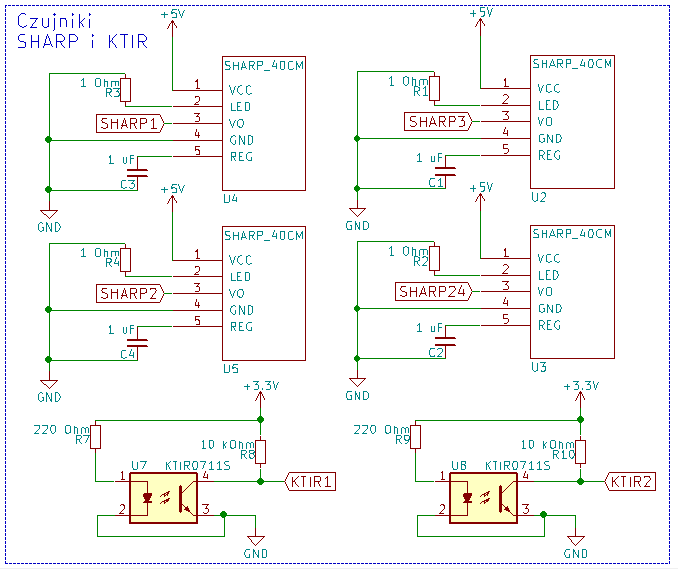
\includegraphics[width=0.8\textwidth]{figures/czujniki}
\caption{schemat Sharpów i Ktirów  \label{fig:czujniki}}
\end{figure}

\subsubsection{Sterowanie silnikami}
Zasilanie silników napięciem 7,4V  odbywa się po przez 2 podwójne mostki H TB6612FNG. Są one łatwe w sterowaniu, wystarczy jeden sygnał PWM kontrolujący szybkość obrotu kół i 2 stany logiczne do obsługi kierunku obrotu. TB6612FNG są mostkami podwójnymi, oznacza to że jeden taki mostek może sterować dwoma silnikami naraz Jednak w celu zwiększenia wydajności prądowej odpowiednie pady zostały ze sobą połączone i wykorzystane do sterowania tylko jednym silnikiem. PWM jest to popularna metoda wykorzystywana do imitowania sygnału analogowego przez sygnał cyfrowy.


\begin{figure}[!]
\centering
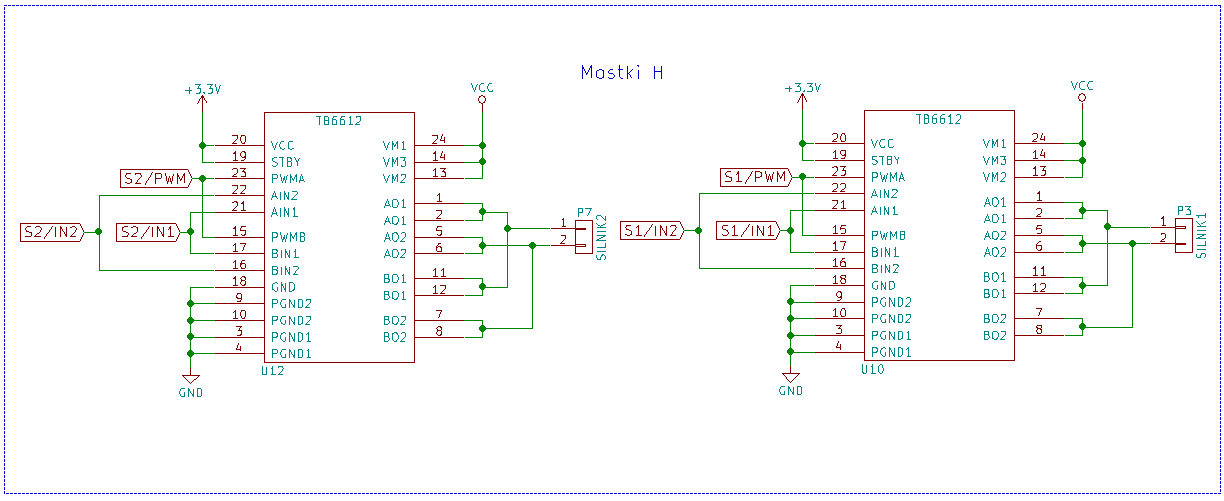
\includegraphics[width=0.8\textwidth]{figures/tb}
\caption{schemat mostków H TB6612FNG  \label{fig:tb}}
\end{figure}

\subsubsection{Interfejs komunikacyjny}
Komunikacja z robotem odbywa się dzięki trzem diodami led, buzzerem, przyciskiem do resetu, modułem startowym, modułem bluetooth oraz programatorem. Jedna dioda LED informuje nas o obecności zasilania w układnie a 2 pozostałe są programowalne. Zostały one wykorzystywane do sprawdzania pracy czujników. Moduł BT połączony za pomocą USART daje nam możliwość startu i stopu robota przez aplikacje na androida napisaną w APP INVENTOR 2. Uniezależnia to robota od modułów startowych podczas testów. Aktualnie w trakcie pisania jest wersja aplikacji pozwalająca ręczni sterować robotem. Moduł startowy jest obsługiwany dzięki prostego wejścia GPIO. Jako programator wykorzystaliśmy ten wbudowany w płytkę nucleo64 którą dostaliśmy w ramach warsztatów. Pozwalał on na wgranie programu na mikrokontroler oraz podglądanie wartości 
zmiennych przy debugowaniu.

PS. Przy projektowaniu PCB z modułem bluetooth warto zwrócić uwagę na zamianę linii Rx i Tx. Aczkolwiek Trochę rzeźby jeszcze nikomu nie zaszkodziło. :)

\begin{figure}[!]
\centering
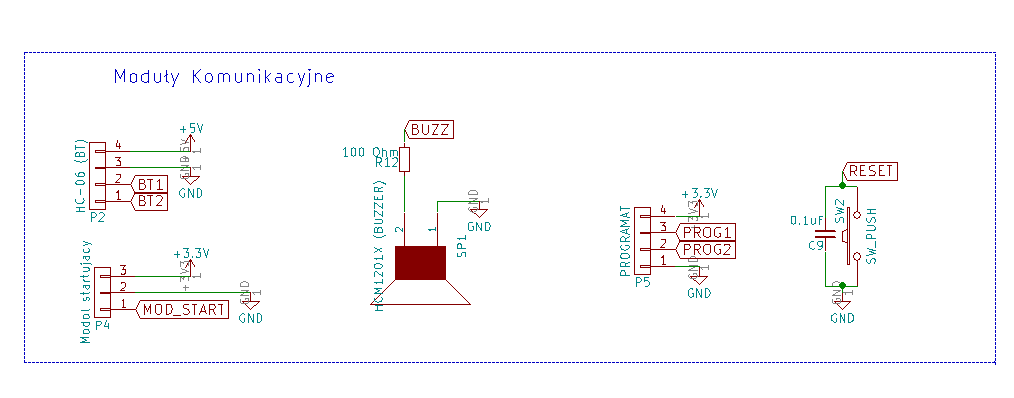
\includegraphics[width=0.8\textwidth]{figures/komunikacyjne}
\caption{schemat modółów komunikacyjnych  \label{fig:komunikacyjnes}}
\end{figure}

\subsubsection{PCB}
Projektowanie płytki PCB również został wykonany programie KiCad. W pierwotnej Białej-Damie Problemem stanowiła dość duża ilość elementów tht, za małe pady w footprintach oraz za wąskie ścieżki. Jednak dzięki doświadczeniu sprzed roku poprawiłem większość błędów. (z wyjątkiem braku zamiany Rx z Tx w BT). Po spaleniu mikrokontrolera dzień przed rozmową kwalifikacyjną do KoNaRu rok temu w tym roku zamówiłem płytkę z strony PCBWay dzięki czemu zaoszczędziłęm masę czasu i nerwów, oraz co najważniejsze zyskałem sordermaskę która chroni procesor przed losowym spięciem ścieżek przez kawałek zapodzianej cyny.

\begin{figure}[tp]
\centering

    \subfloat[schemat płytki pcb]{%
     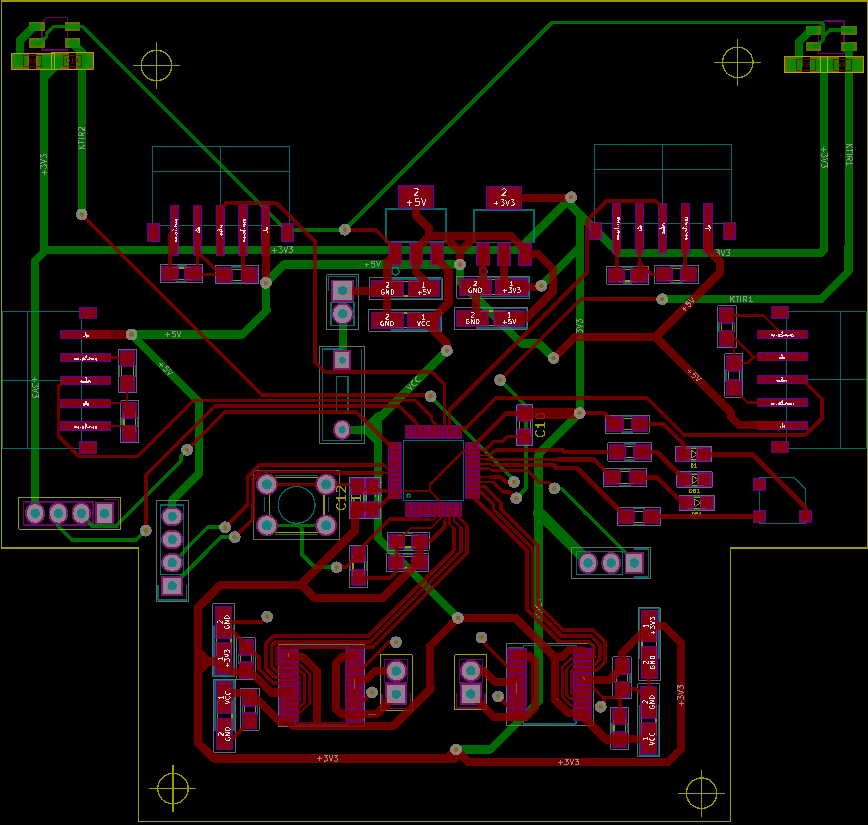
\includegraphics[width=0.4\textwidth]{figures/pcb}
    } %Miedzy tymi obrazkami nie ma przerwy, wiec beda zestawione poziomo
    \hspace{0.4cm}
    \subfloat[wytrawiona płytka z przylutowanymi elementami]{%
     \includegraphics[width=0.4\textwidth]{figures/pcbzc}
    }%Ponizej jest przerwa, wiec nastapi przejscie do nowej linii


    \subfloat[wytrawiona płytka przód]{%
      \includegraphics[width=0.4\textwidth]{figures/pcbzp}
    }
    \hspace{0.4cm}
    \subfloat[wytrawiona płytka tył]{%
      \includegraphics[width=0.4\textwidth]{figures/pcbzt}
    }

    
    \caption{płytki PCB}
  \end{figure}%




\subsubsection{Podsumowanie}
Podczas projektowania elektroniki wiele rzeczy zostało poprawione po poprzedniej wersji robota przez co nie ma większych błędów. Doświadczenie zdobyte rok temu naprawdę wiele pomogło. Jedynym poważnym błędem było podłączenie Bluetootha. Jeżeli chodzi o założenia elektroniczne to uważam że w robocie znajduje się za mało środków komunikacji z człowiekiem. Jak wszyscy ciągle się uczymy.

\subsection{Program}
Program do naszego robota został napisany w języku C, jest najpopularniejszy język do programowania mikroprocesorów i ma najwięcej wsparcia. Dla nas zaletą było również to że składnie C znaliśmy już wcześniej. Środowiskiem do niego był 'system workbench for STM32'. Środowisko to jest kompatybilne z programem STM32CubeMX więc kwestia konfiguracji robota sprowadzona została do wyklinania paru przyciskach w Cubie. Oba programy są darmowe 

\subsubsection{Konfiguracja peryferii}
Taktowanie BD2 nastawione jest na maksymalną wartość tzn. 48 MHz. Częstotliwość bramki PWM wynosi 16 kHz i posiada 1000 stopni wypełnienia. Robot wykorzystuje przerwania systemowe wykonujące się z częstotliwością 100 Hz sprawdzających czy przetwornik ADC nie wykrył białej linii. Robot obsługuje również komunikacje USART dzięki której możliwe jest sterowanie przez moduł bluetooth HC-06.

\subsubsection{Algorytm sterowania}
Sterowanie Robotem odbywa się na bardzo prostej koncepcji. Nieskończona pętla w której sprawdzany jest odczyt z wszystkich czujników i podejmowanie działań zależnie od tego gdzie znajduje się robot przeciwnika. Zaimplementowane są parę rodzai czynności: kręć w lewo/prawo, jedź do przodu i lekko w lewo/prawo, jedz prosto, jedz mocno w lewo/prawo(jedno koło od tyłu) oraz start stop i cofani w przypadku wykrycia linii. Rodzaj wykonywanej czynności zależy od odczytu pozycji przeciwnika oraz możliwości wykrycia białej linii. Została dodana również domyślny kierunek obrotu w przypadku stracenia przeciwnika z oczu. Wybiera się on przed walką przez zakrycie ręką prawego lub lewego czujnika. Pozwala to na jak najszybsze znalezienie przeciwnika przez obrót w dobrą stronę na starcie walki.


\section{Podsumowanie}
Robot Biała-Dama wystartował na Robotic Arena 2016. Niestety nie zadowoliły mnie jego osiągnięcia i uważałem że z tego projektu da wycisnąć się więcej. Fakt spalenia mikroprocesora i niepowodzenie w rozmowie kwalifikayjnej do koła umocnił mnie w przekonaniu że trzeba zrobić tego robota od nowa. Tym razem sam zająłem się reaktywacją projektu. BD2 jest tym czego nie udało się osiągnąć rok temu. Wystartował w Robotic Arenie 2017 bez żadnych problemów. Niestety wyjść z grupy się nie udało ale 2 wygrane walki już satysfakcjonują. Aktualnie największym problemem robota jest lekki pług co jest do poprawy na następne zawody. Planuje również dodać sterowanie przez aplikacje. 

\section{Materiały źródłowe}
\begin{enumerate}
%
\item Warsztaty robotyczne KoNaRu - podstawowe informacje: co? gdzie?
jak? szukać informacji?, oraz obsługa niezbędnych programów.
%
\item Datasheet - informacje odnośnie parametrów i poprawnego podłączenia
podzespołów
%
\item Froum Forbot.pl - szukanie inspiracji i rozwiązywanie niejednego problemu
%
\item Grupa Warsztatowa na której zawsze można było uzyskać pomoc na
każdym etapie konstrukcji
%
\item Opiekun grupy Bartłomiej Kurosz który zawsze z chęcią pomagał przy
problemach. Przy pierwszej wersji Białej-Damy
%
\end{enumerate}



\begin{figure}[tp]
\centering

    \subfloat[cały]{%
     \includegraphics[width=0.9\textwidth]{figures/caly}
    } %Miedzy tymi obrazkami nie ma przerwy, wiec beda zestawione poziomo
    
    \subfloat[bok]{%
     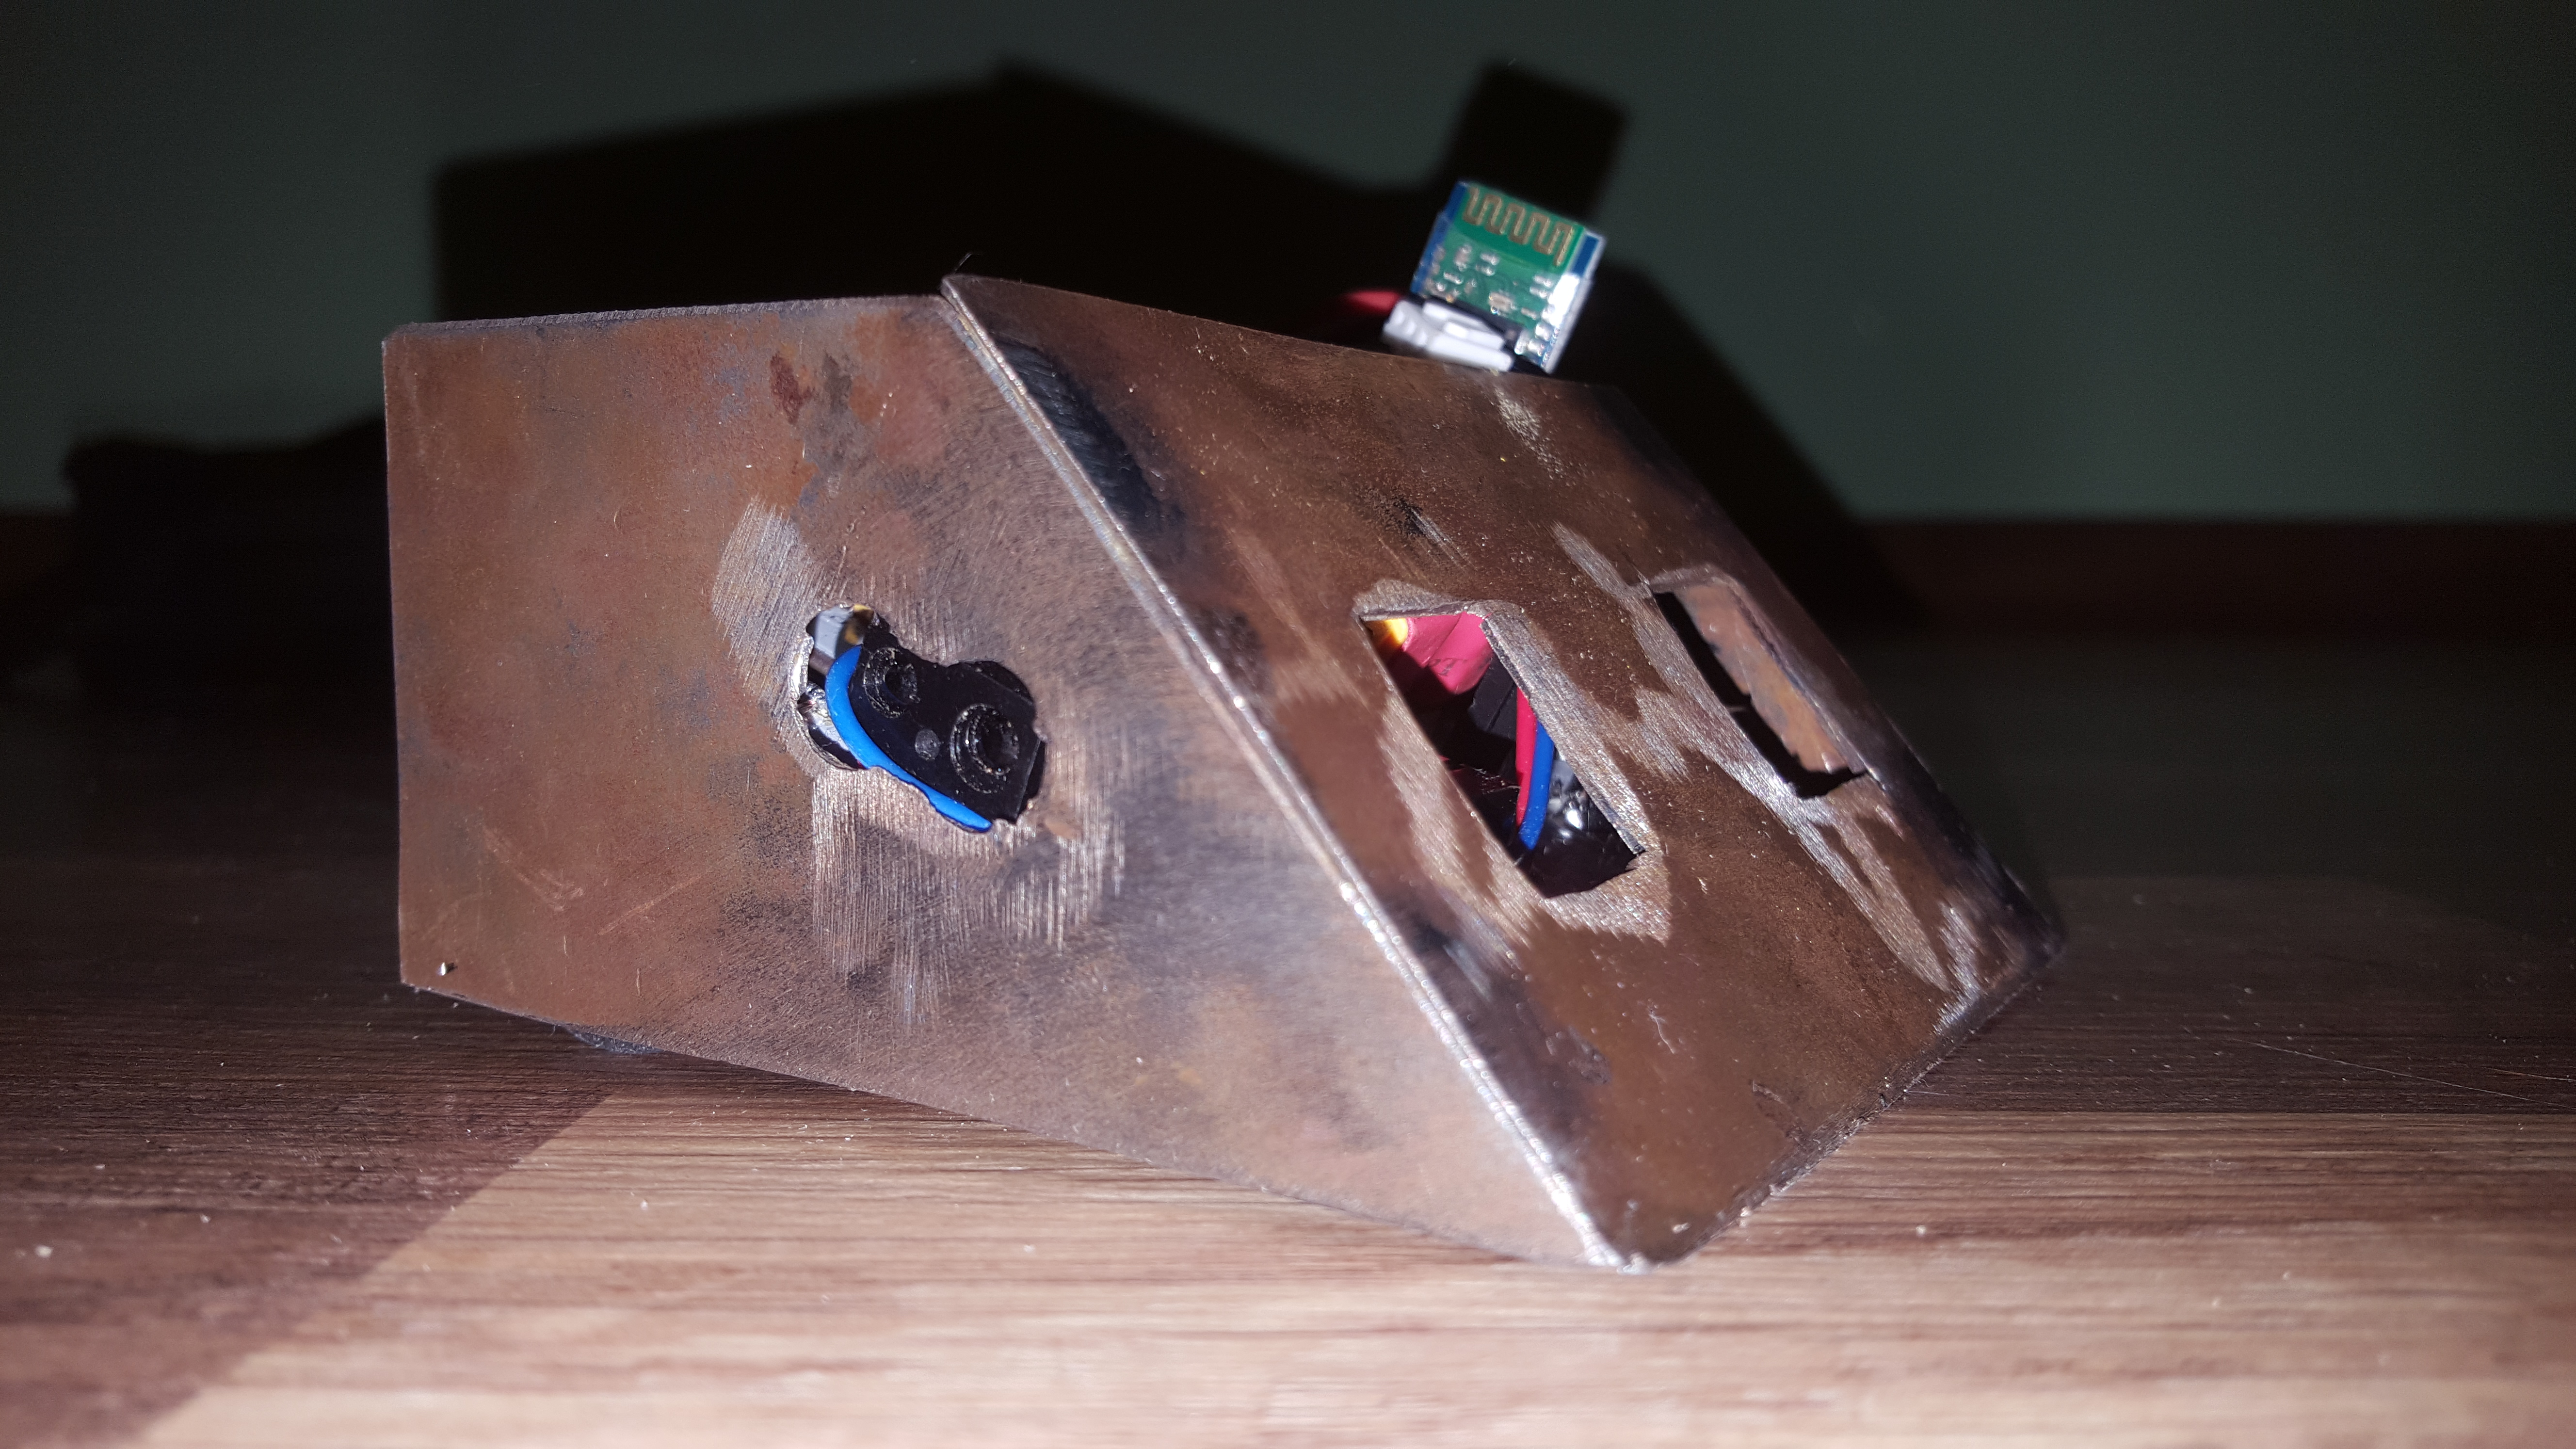
\includegraphics[width=0.9\textwidth]{figures/bok}
    }%Ponizej jest przerwa, wiec nastapi przejscie do nowej linii
    
    \subfloat[góra]{%
      \includegraphics[width=0.9\textwidth]{figures/gora}
    }

  
    \caption{Zdjęcia BD2}
  \end{figure}%


\bibliographystyle{plunsrt}
\bibliography{mybib}
\clearpage



\end{document}
